\newpage

\section{Deep Neural Network Viewer}
\label{sec-dnnviewer}

Deep Neural Network Viewer (DNN Viewer) is a graphical user interface (GUI) showing at the same time the structure, the parameters (weights, intercepts...) and the performance on test data. It is based on the following observations:
 \begin{itemize}
     \item As underlined in \ref{sec5}, activations, saliency (see \ref{sec2}) and occlusion maps, and adverse examples (see \ref{sec3}) provide a very focused views on a single unit or a single layer within a network. However, such views of the DNN do not show overall structure and performance of the network.
     \item The atlases of \ref{sec4} and the embeddings of \ref{sec5} provide an answer to one missing dimension: a global assessment of the unit, layer or network over a full test dataset. But they are missing a representation of the architecture of the network and are not able to show dependencies between neuron units. 
     \item Many available online tools to visualize a DNN are describing the network graph structure, they are not displaying the weights nor assessing the current performance. Among these tools, we may cite Netron (\cite{roeder2020}) which is very comprehensive when it comes to describe the network architecture and supports many formats (Tensorflow, Torch, Caffe...). 
     \item Tensorflow Playground (\cite{tf-playground2020}) goes in the direction of overall network interpretability but is very limited and constrained on network topologies.
     \item Tensorboard provides a mix of structure presentation (Graphs tab), current training parameters (Distributions and Histograms tabs) and performance (Images tab) but there is no link between each of these.
 \end{itemize}

With the DNN Viewer, our aim is to facilitate inspection of the network, to understand the relationship between units, layers and performance on test data. Our intuition is that each neuron power lies within the inter-relationship with other units, and must be evaluated with data samples related to the task accomplished by the model. Also, interpretation cannot be based exclusively on either singular values (i.e. some unit weight or activation), or aggregated values (i.e. layer weights histogram, class average activation), that is why a GUI providing access and switch between these views is very useful to the person in charge of the interpretation.

\ul{As a first step}, 
the DNN Viewer capabilities are limited to \ul{Keras Sequential models} and its main target is images. It can be used with other type of datasets but the displays are then less interesting. 
It will be later extended to other architectures. \ul{DNN Viewer is to be used as a DNN pedagogical tool, and will not scale on medium to large models} since the computation required is too long for an interactive GUI; however we could modify the implementation to only show a section of the DNN and thus limit the required computing load.

The DNN Viewer has been successfully tested with various image classifiers and generative adversarial networks (GAN).

Remaining of this chapter is organized as follows. First a quick overview of the functionality, then some details on the architecture and implementation, and eventually some typical use case and findings.


\subsection{Overview}
\label{dnn-viewer-overview}


DNN Viewer is a Web browser application that is loading from files a sequence of models in over training epochs, and displaying several views. The screen is divided in three main sections. The top section contains the forward and backward buttons to select the epoch to be displayed. Middle section is the main view on the network with a side panel showing network properties. Bottom section has four quadrants showing the input test data, layer properties, unit properties and activation maps.

\begin{figure}[H]
    \centering
    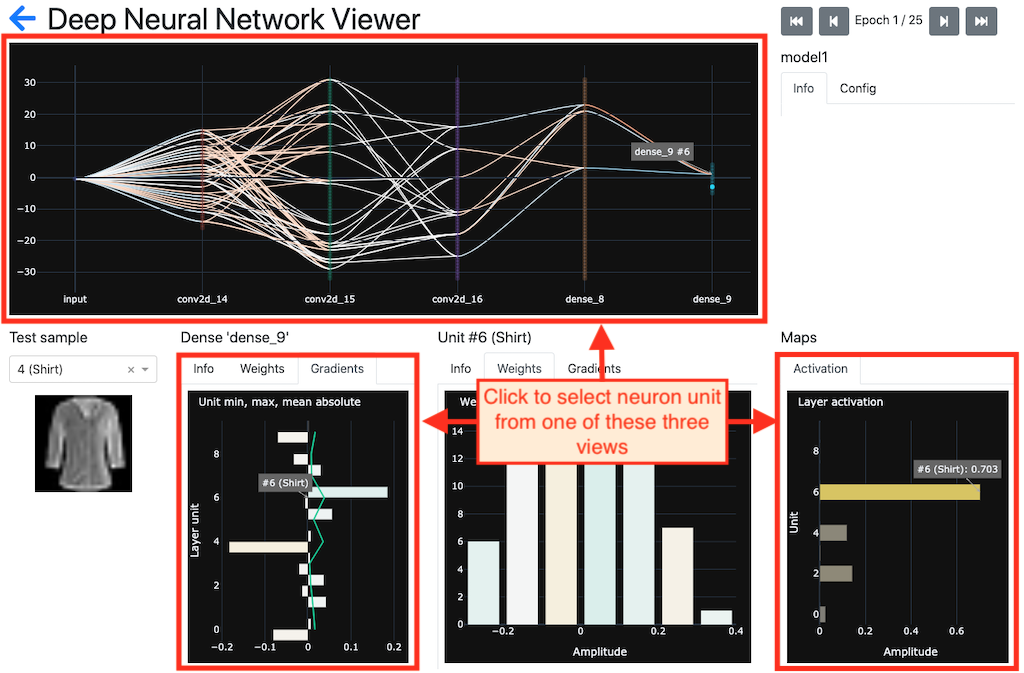
\includegraphics[scale=0.4]{images/dnn-viewer/dnnviewer-selection.png}
    \caption{DNN viewer three panels, from the top panel is selected the training epoch}
    \label{fig:dnn-viewer-top}
\end{figure}

The link between these views is the currently selected layer unit. Selection is made either on the central network view or on the layer weights or gradients figure, or on the layer activation figure (in case of a Dense layer). The selection on the central view will set the layer and unit, whereas the selection on the other views will only update the currently selected unit within the layer. 


\subsubsection{Loading a model}

Model selection is performed through the user interface on the initial page shown on Figure \ref{fig:dnn-viewer-model-selection}.

\begin{figure}[H]
    \centering
    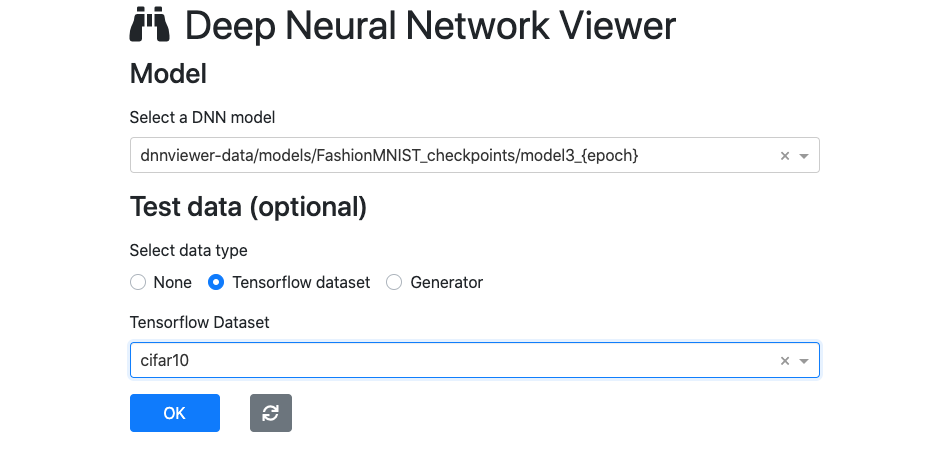
\includegraphics[scale=0.3]{images/dnn-viewer/ModelSelection.png}
    \caption{Model selection in the DNN Viewer GUI}
    \label{fig:dnn-viewer-model-selection}
\end{figure}

The supported model file formats are  HDF5 and Tensorflow checkpoint. Checkpoints can be used as sequences over training epochs if a naming pattern is detected (default pattern is \verb|{model_name}_{epoch}| as illustrated on Figure \ref{fig:dnn-viewer-model-selection} in which the sequence for "model2" is selected).

\subsubsection{Central network view}

This central view is providing at the same time the network architecture and the connections between layers. For each of these two aspects the complexity is raising very quickly with the number of layers, that is why a simplified view is built based on the following choices:
\begin{itemize}
    \item Only the main layers with weights are displayed : fully connected, convolutional layers. The activation, dropout, pooling, batch normalization, upsampling, reshape layers are appended as attributes to previous or following layers. The goal is to decrease the total number of plotted layers and avoid clutter.
    \item Layer connections are showing the main multiplicative weights, starting from the selected layer unit. This algorithm is detailed in \ref{sec-dnnviewer-implementation-topn-connections}
\end{itemize}

This Visualization is very important it must provide the user with some intuitions on what is happening in this dense and complex graph.

\subsubsection{Detailed views}

The bottom panel contains 4 quadrants with detailed views: test data input, layer, unit and maps.

For each of these, there may be alternative views selected through tabs. For example, the layer and unit quadrants have descriptive information in the "Info" tab, and current training parameters in the "Weights" and "Gradients" tab. 

The layer figures are showing three quantities for each of the unit in the layer: minimum, maximum and mean absolute of the values (weights or gradients).

\begin{figure}[H]
    \centering
    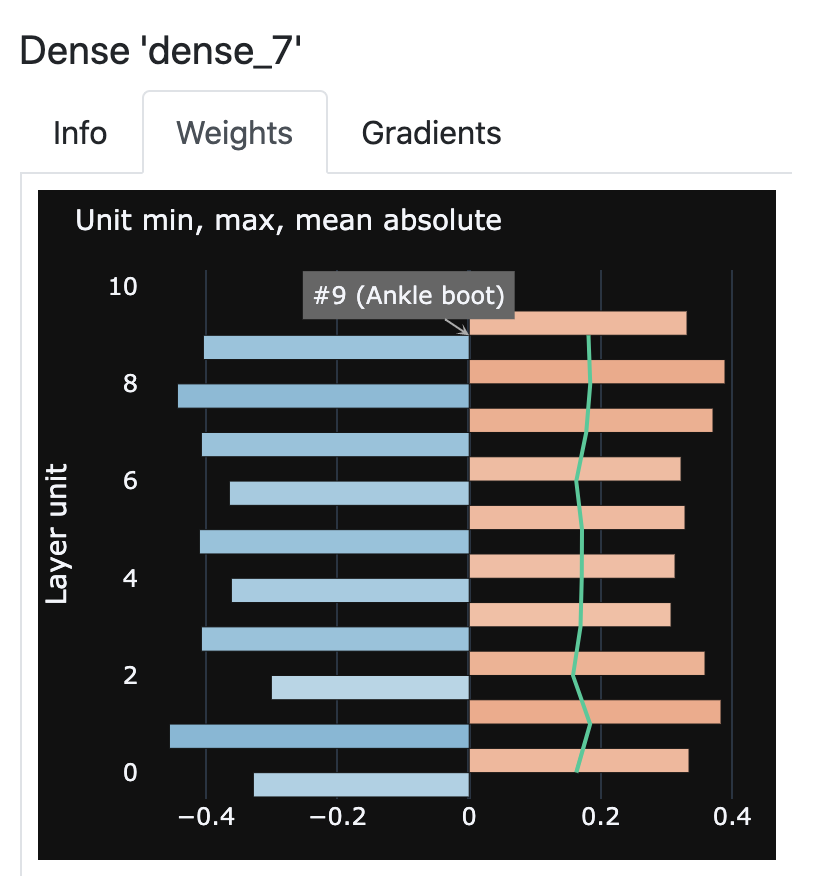
\includegraphics[scale=0.3]{images/dnn-viewer/LayerMinimax.png}
    \caption{Layer view showing min (blue bars), max (red bars) and mean absolute (green multiline) for each of the layer units}
    \label{fig:dnn-viewer-layer-minimax}
\end{figure}


The layer unit figures are different for Dense and convolutional layers: for Dense they are histograms, for convolutional the first filters of the unit are shown.

\begin{figure}[H]
    \centering
    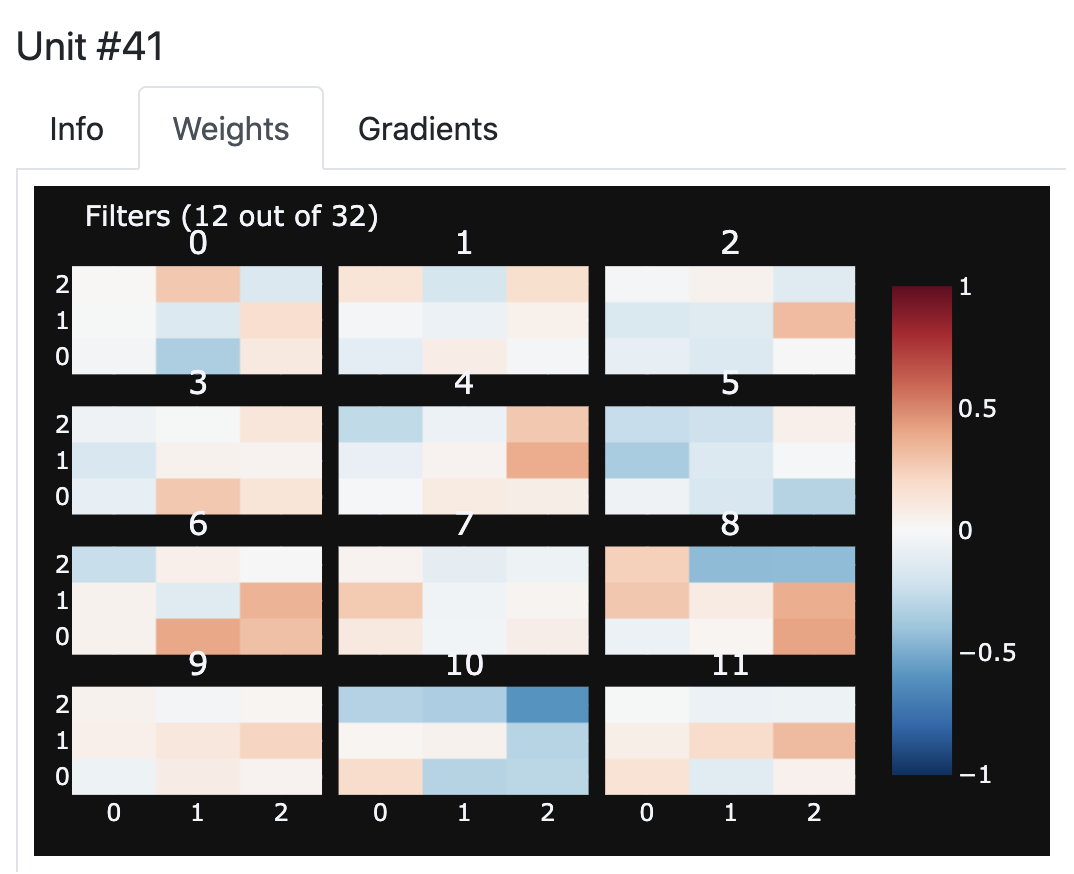
\includegraphics[scale=0.3]{images/dnn-viewer/ConvoFiltersWeights.png}
    \caption{convolutional unit filter view}
    \label{fig:dnn-viewer-unit-convo-filters}
\end{figure}

For the time being, maps are restricted to activation maps, but the saliency maps are in the road-map. 



\subsection{Implementation}
\label{sec-dnnviewer-implementation}


\subsubsection{Software stack (system architecture)}

Starting from a simple visualization on a Jupyter notebook, the DNN Viewer evolved to a client-server web application that reflects its origins and its audience, Data Scientists. The language is Python, the server framework is Plotly Dash, the main dependency is Tensorflow for reading models and evaluating gradients and activations. Dash is generating the client code that relies on Plotly.js and React.js. On the server side, Dash relies on the light web HTTP server Flask. The software stack is depicted on Figure \ref{fig:dnn-viewer-archi1}. The programming paradigm of Dash is tightly linked to the one of React.js: callbacks are fired in reaction to events on the user interface.

Currently, the application code is not state less (as in RESTful paradigm): the model is loaded once, linked to its graphical representation and stays on the server. Moreover, there is no management of user sessions, meaning that only a single user is handled, one model may get loaded at a time. 


\begin{figure}[H]
    \centering
    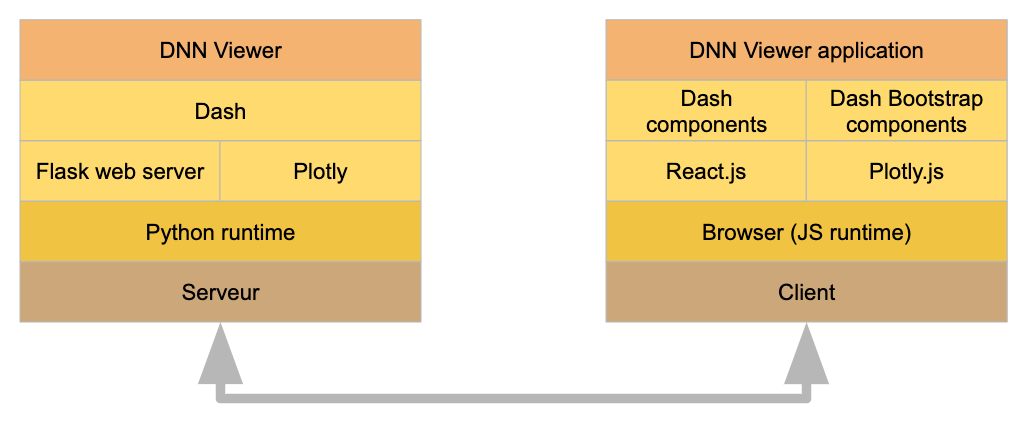
\includegraphics[scale=0.3]{images/dnn-viewer/Architecture.png}
    \caption{DNN viewer software stack}
    \label{fig:dnn-viewer-archi1}
\end{figure}

Main advantages of this environment are a single language (Python) to perform at the same time server processing and client side interaction (necessary Javascript is generated by Dash), and the integration with Plotly, a powerful evolution of Matplotlib. Finally, the install is easy through package management by Pip3.

Drawbacks are a lack of control over the client side events, some limits to Dash when the application has multiple pages (Dash requires all callbacks and bindings to be declared at initialization), and a large dependency on Dash as an open source project that is not so widespread.


\subsubsection{Software architecture}

As many Web applications, the DNN Viewer application is a set of pages that are routed based on events. In Dash, all pages are instantiated at startup in order to create the callbacks. This is done from the main script of DNN Viewer.

The pages are relying on three other components displayed on \ref{fig:dnn-viewer-archi2}:
\begin{itemize}
    \item The Dash application
    \item The \textit{Grapher} which is responsible for the graphical representation of the network and holds a collection of layers
    \item The model sequence which is performing all tasks related to the original model (managing a single or sequence of models, loading the models and creating the layer in the \textit{Grapher}, gradient and saliency computation)
\end{itemize}

\begin{figure}[H]
    \centering
    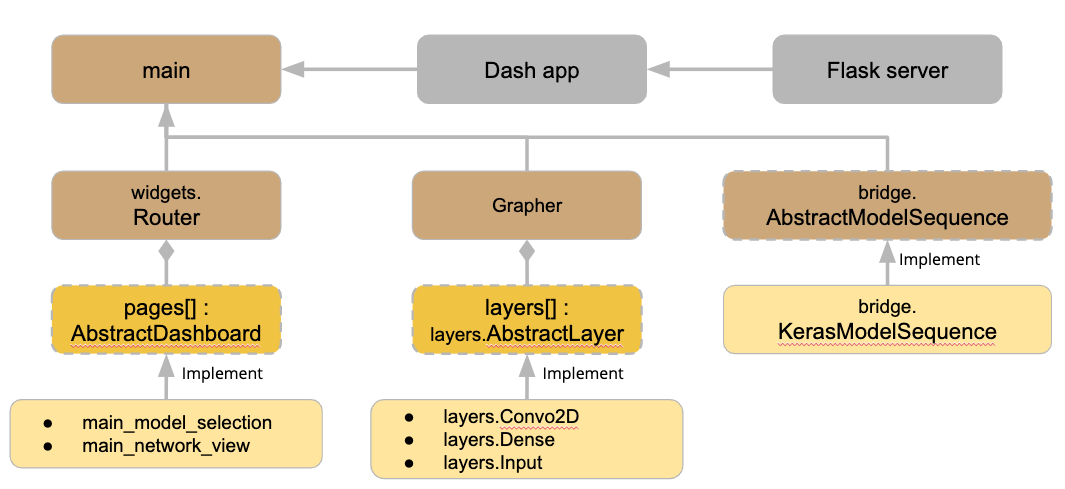
\includegraphics[scale=0.3]{images/dnn-viewer/Architecture2.png}
    \caption{DNN viewer software architecture}
    \label{fig:dnn-viewer-archi2}
\end{figure}


DNN Viewer could be extended to support Pytorch models creating a class specialization of \\
bridge.AbstractModelSequence similar to bridge.KerasModelSequence.


\subsubsection{Visualization of the main connections between layers}
\label{sec-dnnviewer-implementation-topn-connections}

As explained in the overview, the connections between layers are shown as a selection of the weights that link units. There are two main constraints on this visualization, -1- it shall not become over complex, i.e. look as spaghetti, and -2- it shall not take too much computation time since it will be computed at each user selection refresh.

The chosen implementation is taking the currently selected layer neuron unit as focal point. When the application is started, the unit corresponding to the target true class of the first data sample image is automatically selected.

From this focal point, the N weights with the highest absolute value are selected, with N between 1 and 4. This is applied on both sides of the unit: downstream and upstream and propagated to layers through backward and forward propagation. This propagation is taking as focal points the units connected from previous layer. Since N connections are shown at each selected unit, the N units connected are then part of the selection for next layer to layer connection plot, the number of connections grows as a \(N^l\) with \(l\) as the number of layers between the initial layer and the current layer. This number grows very quickly and will simultaneously saturate the visualization and slow down the plot. In order to limit the number of shown connections between two layers, the number of selected (active) units at each layer is arbitrarily capped at 32.

\begin{figure}[H]
    \centering
    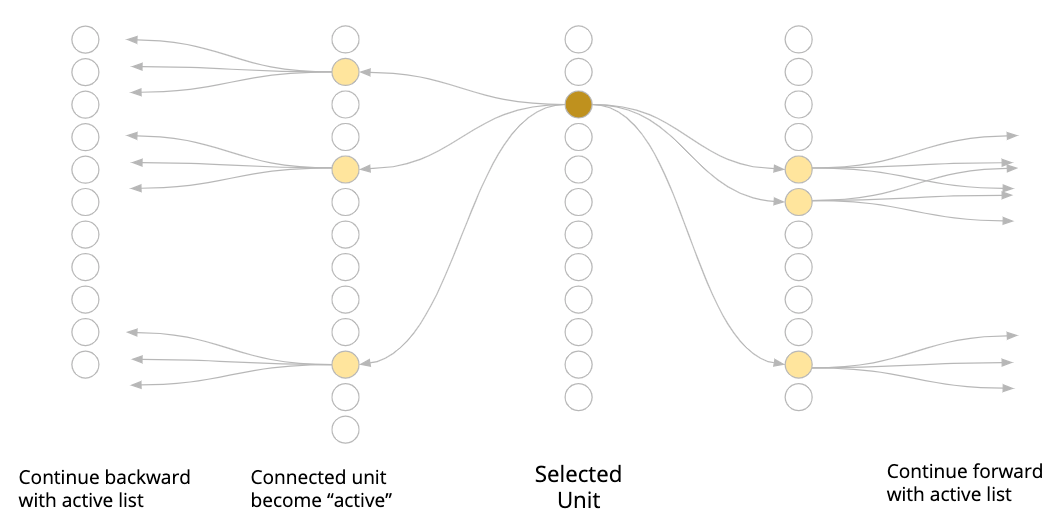
\includegraphics[scale=0.4]{images/dnn-viewer/TopNConnections.png}
    \caption{DNN viewer algorithm to select connections to plot}
    \label{fig:dnn-viewer-topn-connections}
\end{figure}

Each unit to unit connection is plotted as a cubic Bezier curve. The weight strength is plotted as the color of the spline using a divergent color map.

Last but not least complication, when a convolutional layer is connected to a fully connected, there is often an intermediate pseudo layer to "flatten" the tensor at the output of the convolutional layer. It means that the is no one to one connection between the convolutional layer dimension and what is seen as an input dimension on the fully connected layer. This is handled by wrapping the connection number when computing the layer to layer connection plot backward. In the forward pass, there is no such issue. This problem is similar to the one of \ref{embeddings-convolutional}.

\textbf{Discussion on the weight selection:}
\begin{itemize}
    \item For each unit, the selected weights to be plotted are the top N in absolute value. We could argue that given the most used activation function today is ReLU and is asymmetric (truncating negative values), the negative contributions are most-likely discarded. However, there is no direct link between negative contributions and negative weights, it depends on the full forward chain of the network, starting from the image stimuli. For these reasons, the activations are totally ignored in this visualization.
    \item Each layer to layer is evaluated independently starting from the "active list", we could think of a cumulative evaluation that might lead to some weight to vanish as the origin layer is far away. This is area for improvement and might help in keeping low the number of plotted connections, replacing the cap to 32 units in the active list above.
\end{itemize}

\subsubsection{Gradient computation with Keras}

Gradients are not available within the saved model files (HDF5 or Tensorflow checkpoint). They are recomputed from the test data performing a forward prediction with a mini-batch of size 128. The result list of gradient tensor is then affected to each of the layers added to the Grapher.


\subsection{Applied interpretability and findings}

From our experience, there are three main ways to use the DNN Viewer (we expect our users to create and ask for others):
\begin{itemize}
    \item Forward to see the evolution of the feature and manifolds learnt by deeper and deeper layers
    \item Backward, starting from the target true class, inspect the main weights backward and cross inspect with the activation maps
    \item Through time across the training epochs to see the evolution of the strong and weak weights and gradients
\end{itemize}

Each of these is exemplified here below

\subsubsection{Forward inspection}

From [\cite{Erhan2009}] and other studies, it is known that first DNN layers tend to select edges similarly to the Sobel filters, second layer is activated on some specific corners of the input shape or manifold, and deeper layers have more and more abstract and trackable activations. This is also amplified by the lower and lower resolution of the activation images following the chain of pooling layers.

\begin{figure}[H]
    \centering
    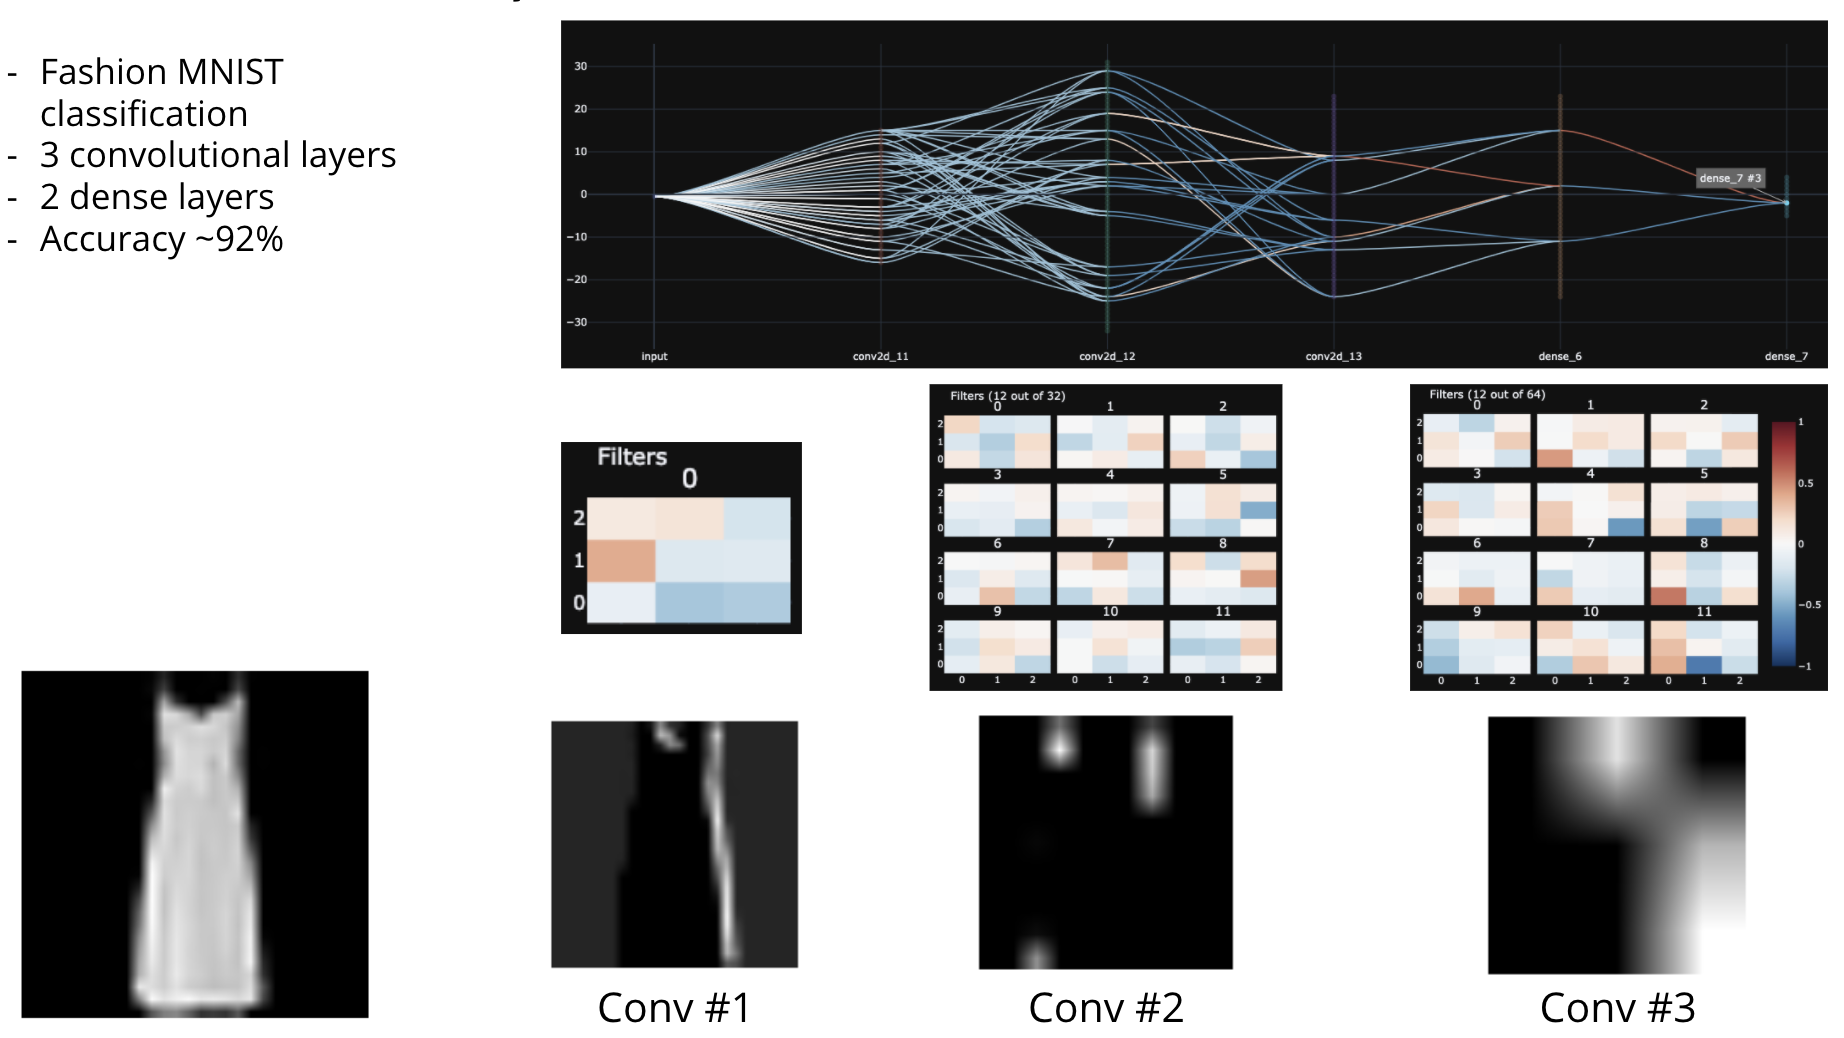
\includegraphics[scale=0.4]{images/dnn-viewer/ForwardDress.png}
    \caption{Forward exploration with a Fashion MNIST dress test image and a simple 5 layer network}
    \label{fig:dnn-viewer-forward-dress}
\end{figure}

Two examples were drawn from a simple DNN to classify Fashion MNIST dataset Figure \ref{fig:dnn-viewer-forward-dress}) and a deeper network handling CIFAR-10 classification (Figure \ref{fig:dnn-viewer-forward-truck}).

The simpler example is showing the progression from edge detection to single region highlights. The larger network is showing a smoother transformation of the input image. The first layer is more like contrast adjustment. The second layer performs the edge detection. On the third and fourth, the truck structure still remains visible but the pooling layer has reinforced the contrast between the image regions of interest and others. On the fifth and sixth, the truck structure is no longer visible and we see some highlighted regions.

\begin{figure}[H]
    \centering
    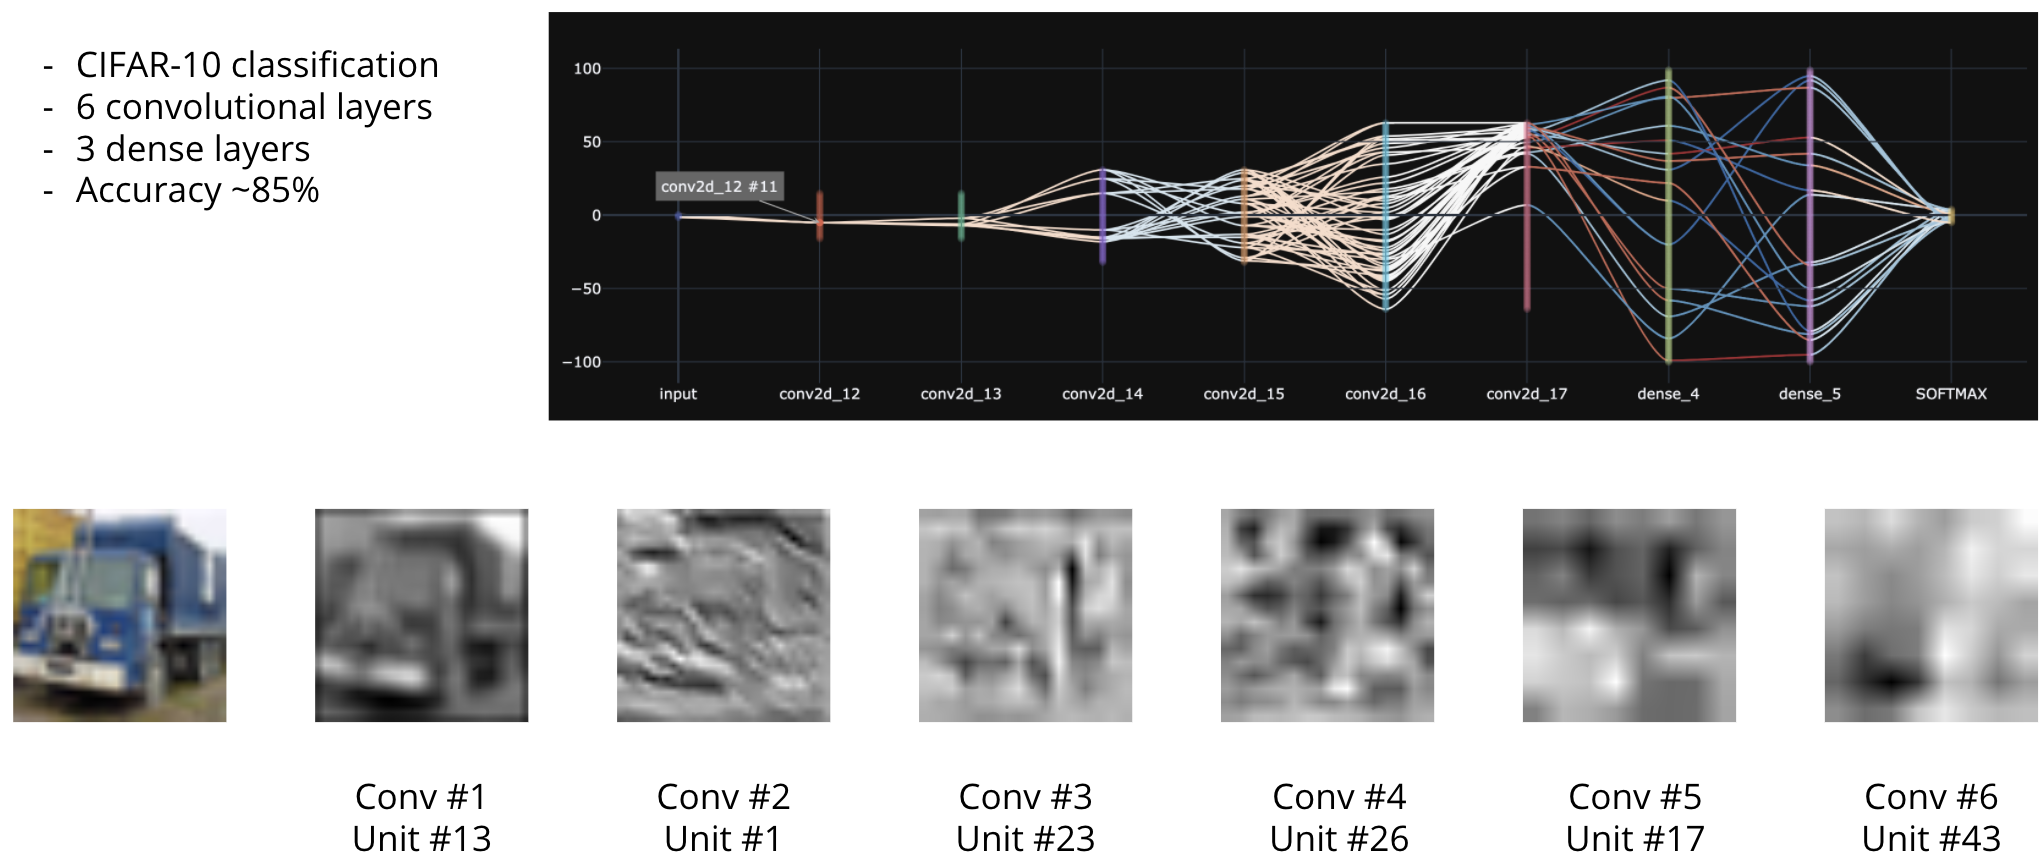
\includegraphics[scale=0.4]{images/dnn-viewer/TruckForward-Large.png}
    \caption{Forward exploration with a CIFAR-10 test image and a large 9 layer network}
    \label{fig:dnn-viewer-forward-truck}
\end{figure}

Something that is visible in the GUI but not on the extracted pictures is the fact that the simpler DNN has low activations and sharp contracts from the first layer, and the selected connections shown are very often negative whereas the larger model has lower contrast and selected connections are often positive.

We conclude from this inspection that the large model could be optimized to reduce its size in both number of layers and number of units per layer.

\subsubsection{Backward inspection}

For this inspection, the test-case is a LeNet5 network optimized in performance and size using ReLU activations, Dropout regularization, see [\cite{lenet5-optimized}]. There are three convolutional and 2 dense layers. 

From the MNIST Digits dataset, a sample three digit has been selected given the output soft-max probability is only 60\%. The probability for the digit five is close to 40\%. This is shown on Figure \ref{fig:dnn-viewer-backward-1}

\begin{figure}[H]
    \centering
    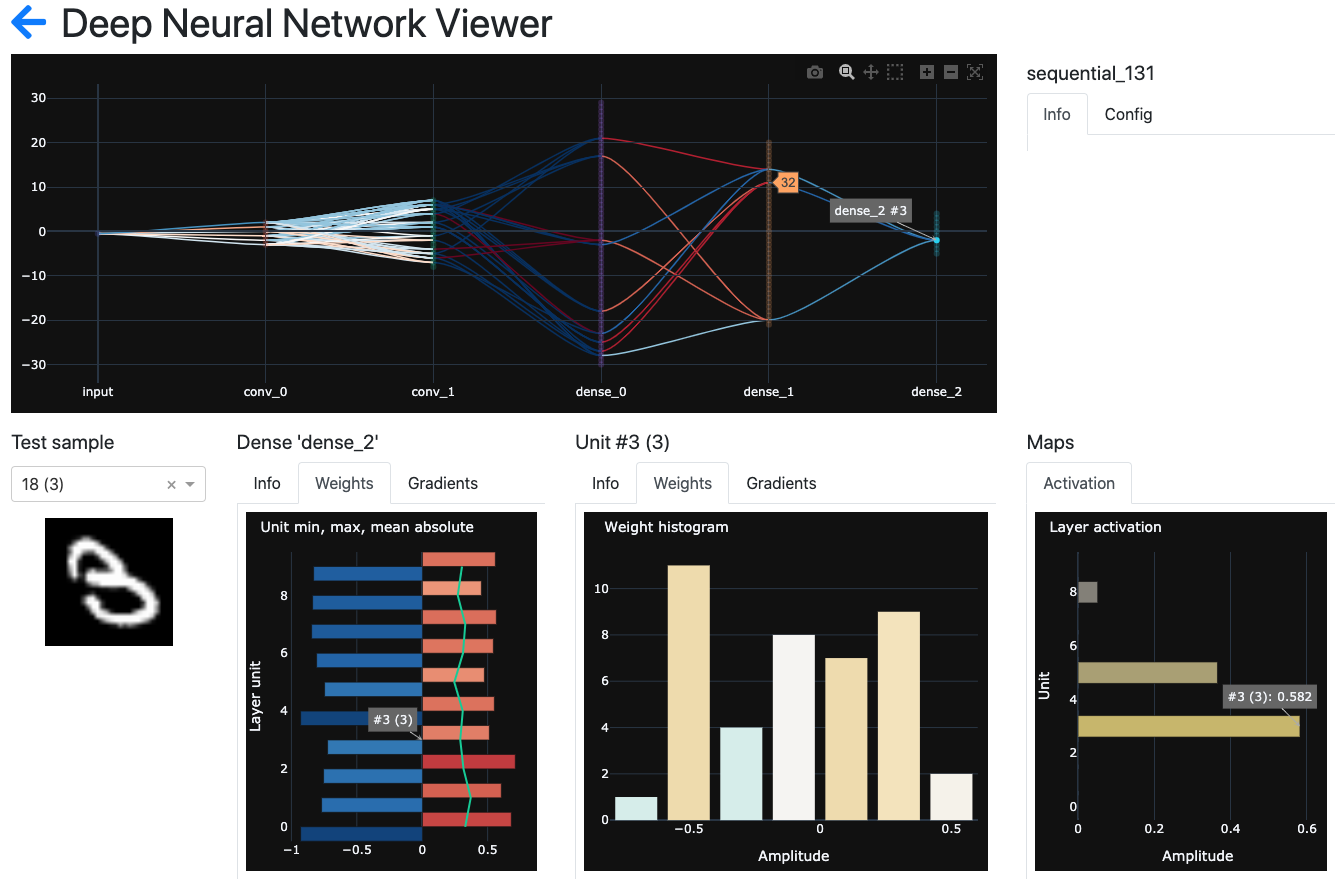
\includegraphics[scale=0.3]{images/dnn-viewer/BackwardThree_1.png}
    \caption{Backward exploration with a LeNet5, output probabilities for a 3}
    \label{fig:dnn-viewer-backward-1}
\end{figure}

On Figure \ref{fig:dnn-viewer-backward-2}, looking at previous layer on the highlighted main negative contribution (unit \#32), it is observed that this unit contributes positively to the softmax probability for the digit 1. Also, there is no activation on this unit for the digit three at the input.

\begin{figure}[H]
    \centering
    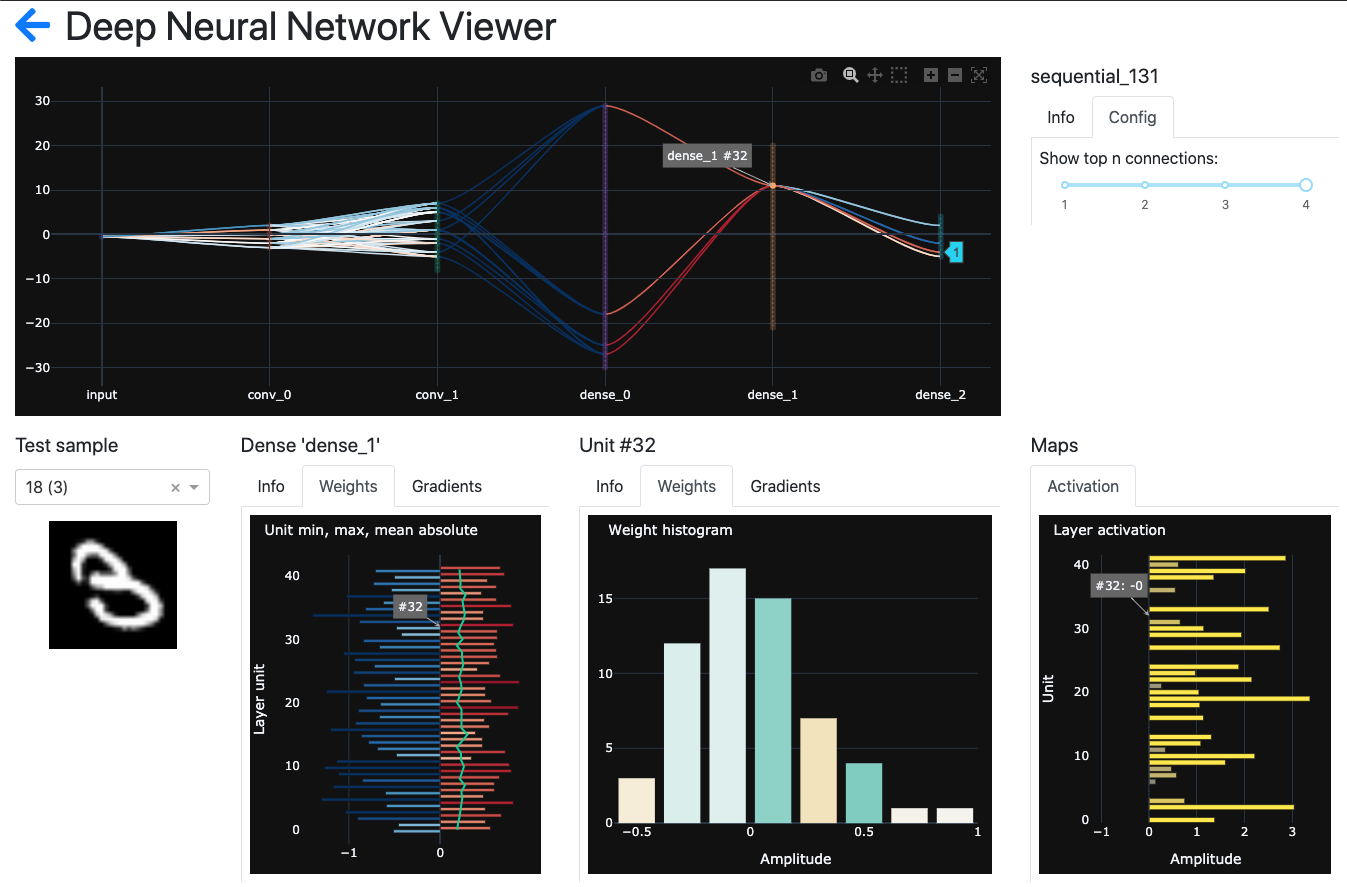
\includegraphics[scale=0.3]{images/dnn-viewer/BackwardThree_2.png}
    \caption{Backward exploration with a LeNet5, layer before the softmax with digit three input}
    \label{fig:dnn-viewer-backward-2}
\end{figure}

The positive contribution to digit 1 of unit \#32 the pre-softmax layer is confirmed on Figure \ref{fig:dnn-viewer-backward-3}

\begin{figure}[H]
    \centering
    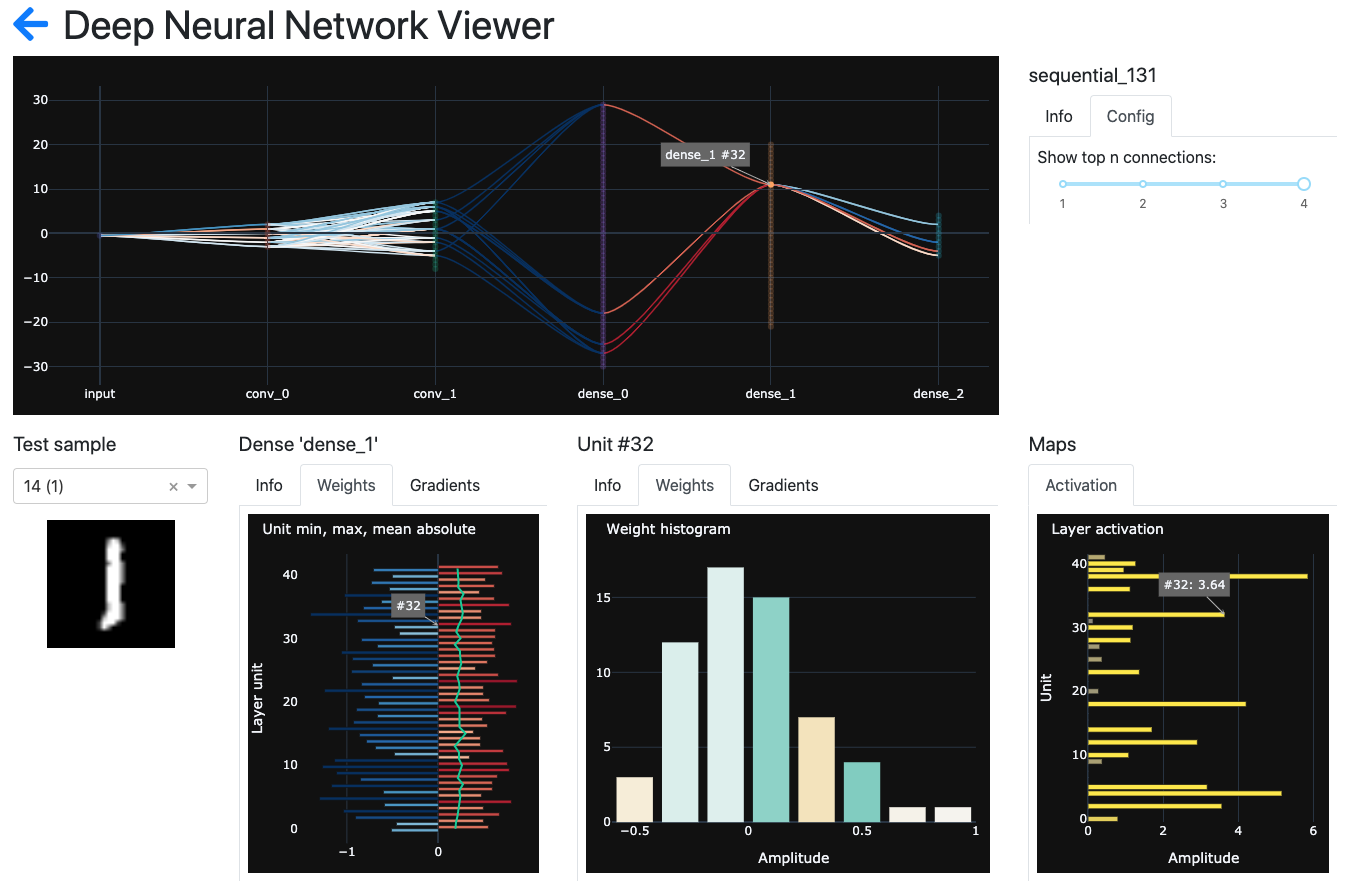
\includegraphics[scale=0.3]{images/dnn-viewer/BackwardThree_3.png}
    \caption{Backward exploration with a LeNet5, layer before the softmax with digit one input}
    \label{fig:dnn-viewer-backward-3}
\end{figure}

Selecting again the digit 3 sample, the main contribution to the digit 5 softmax probability is inspected: unit 39 of the pre-softmax layer, Figure \ref{fig:dnn-viewer-backward-4}. The activation of the input digit three is measured to be quite high for on this unit.

\begin{figure}[H]
    \centering
    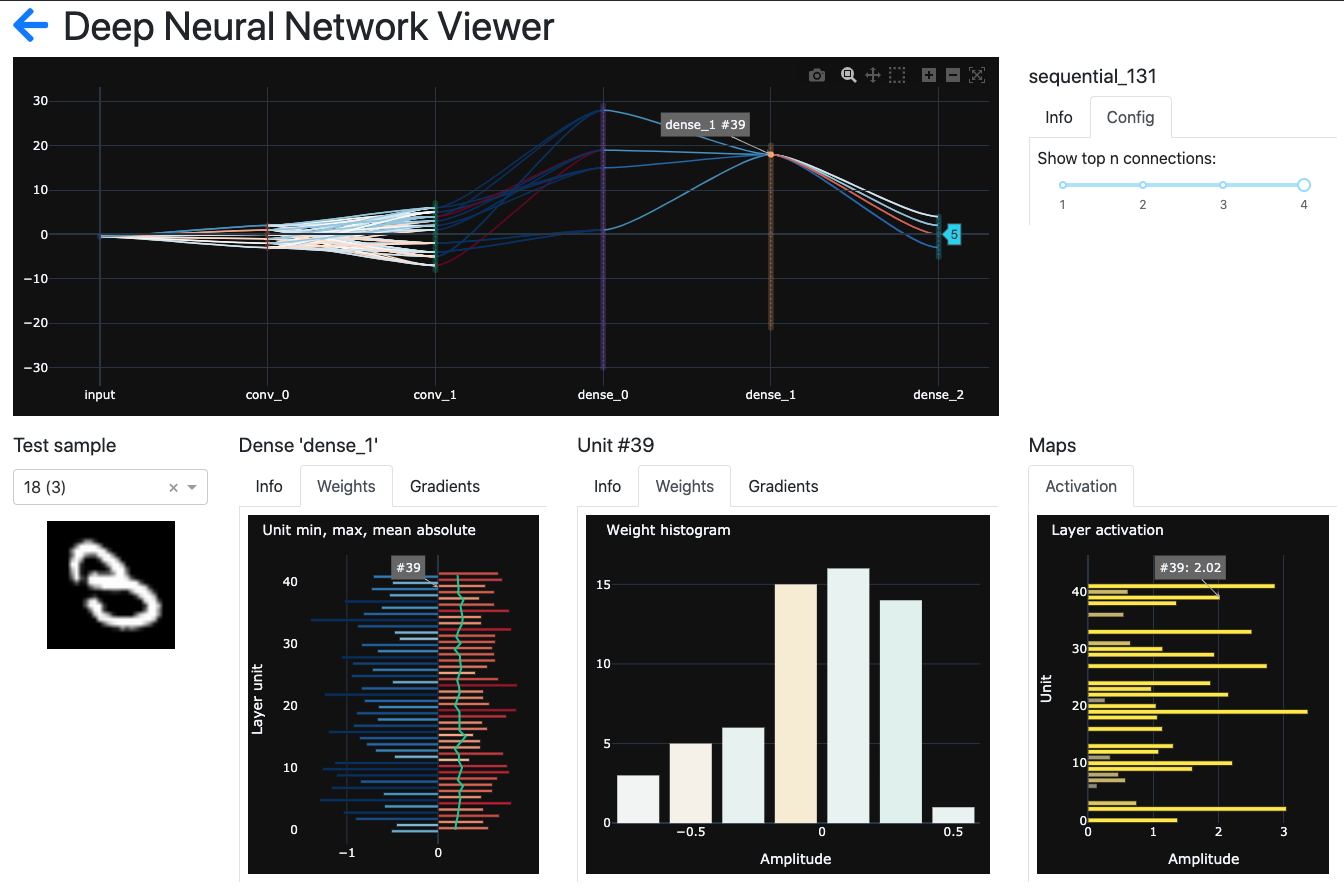
\includegraphics[scale=0.3]{images/dnn-viewer/BackwardThree_4.png}
    \caption{Backward exploration with a LeNet5, layer before the softmax, main positive contribution to digit five}
    \label{fig:dnn-viewer-backward-4}
\end{figure}

Jumping to the last convolutional layer, unit \#0 is selected. It shows a activation on two horizontal bars of the input three, Figure {fig:dnn-viewer-backward-5}. There seems to be a positive contribution to the softmax for digit three through unit \#31 of pre-softmax layer and a negative contribution through unit \#4 of the same layer.

\begin{figure}[H]
    \centering
    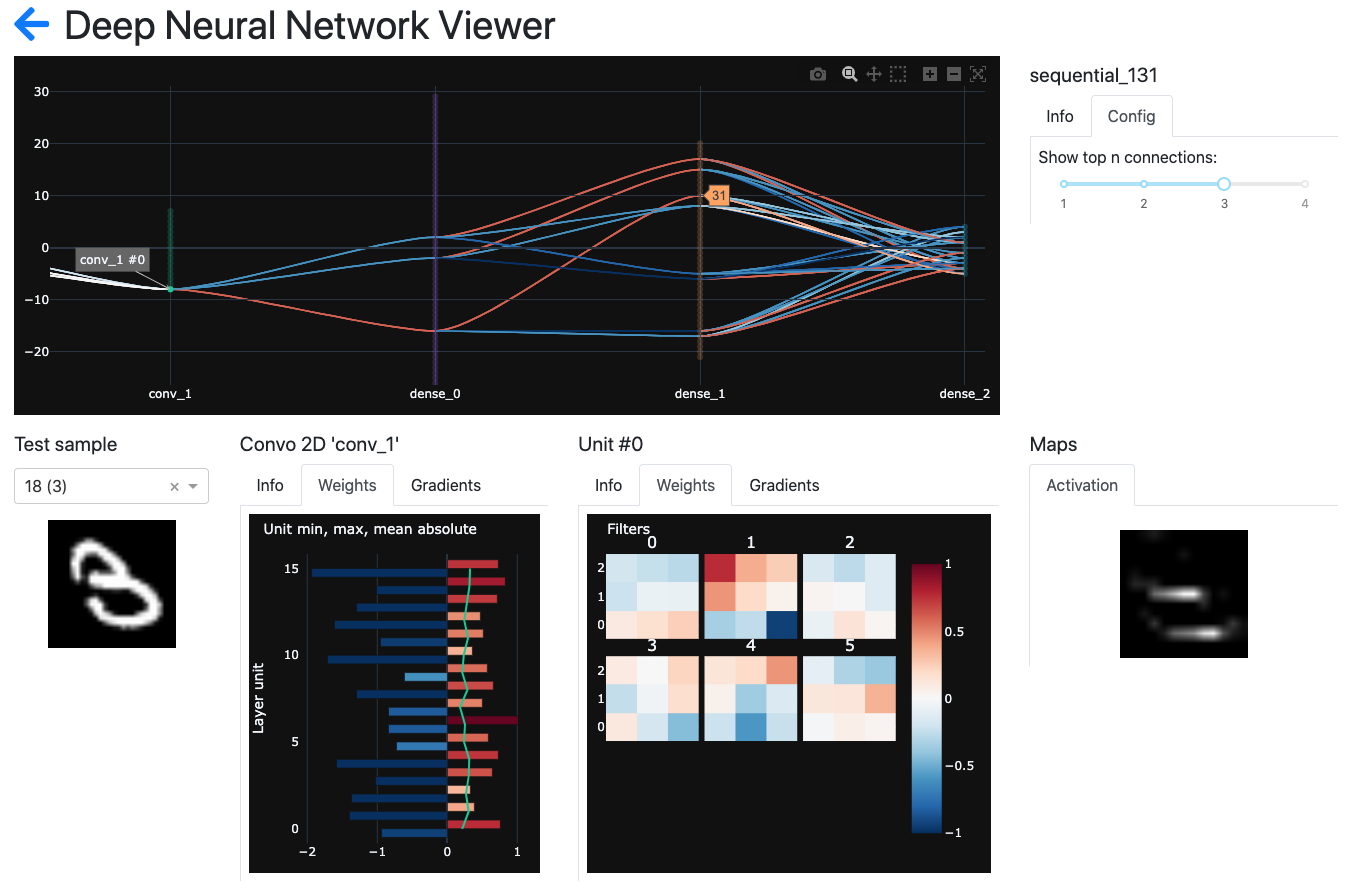
\includegraphics[scale=0.3]{images/dnn-viewer/BackwardThree_5.png}
    \caption{Backward exploration with a LeNet5, last convolutional layer, unit \#0}
    \label{fig:dnn-viewer-backward-5}
\end{figure}

The positive contribution is confirmed on Figure \ref{fig:dnn-viewer-backward-6}. The negative contribution is not activating on the input digit three, that's probably the action of the ReLU activation function, Figure \ref{fig:dnn-viewer-backward-7}.

\begin{figure}[H]
    \centering
    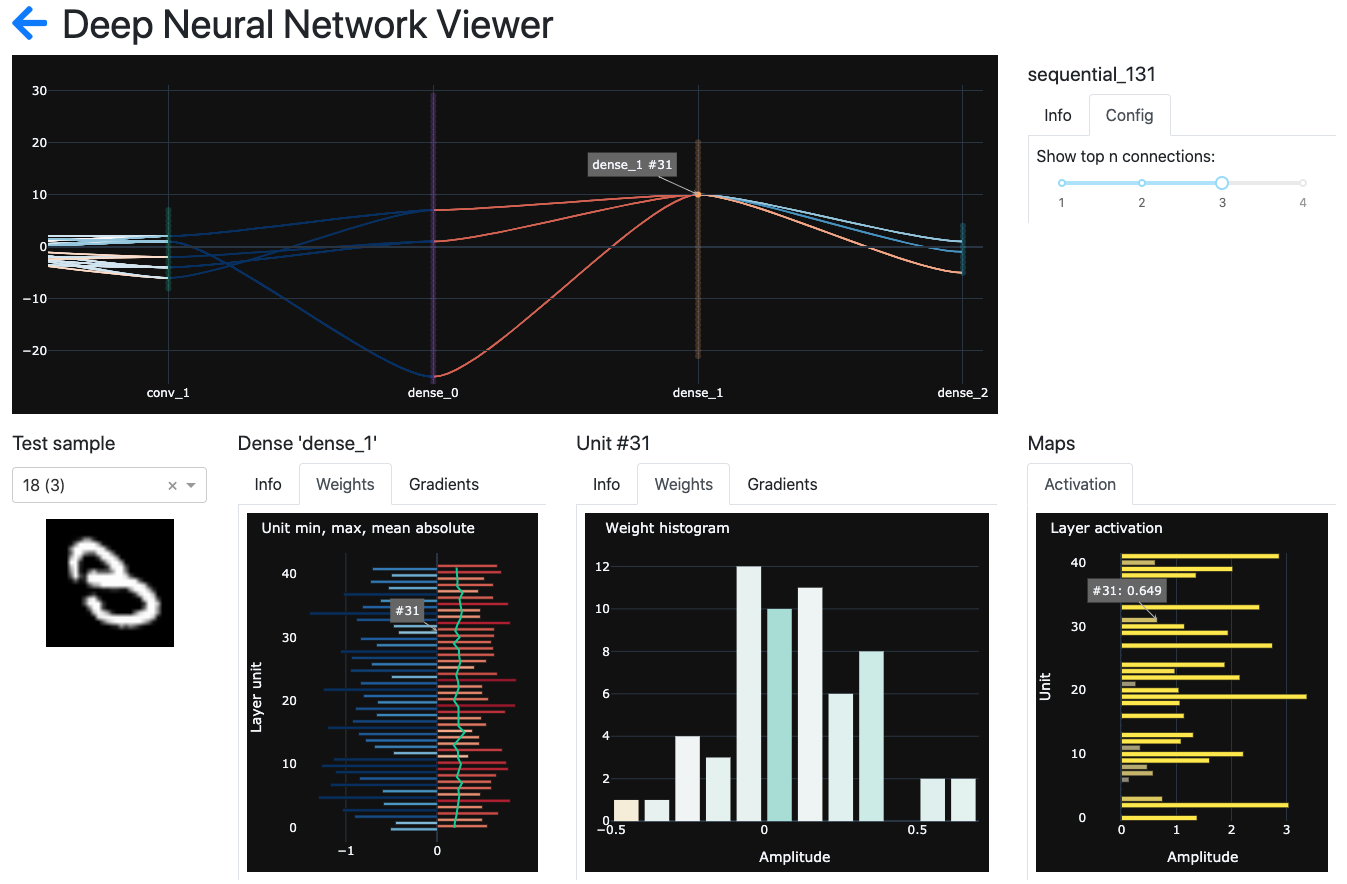
\includegraphics[scale=0.3]{images/dnn-viewer/BackwardThree_6.png}
    \caption{Backward exploration with a LeNet5, pre-softmax layer, unit \#31}
    \label{fig:dnn-viewer-backward-6}
\end{figure}

\begin{figure}[H]
    \centering
    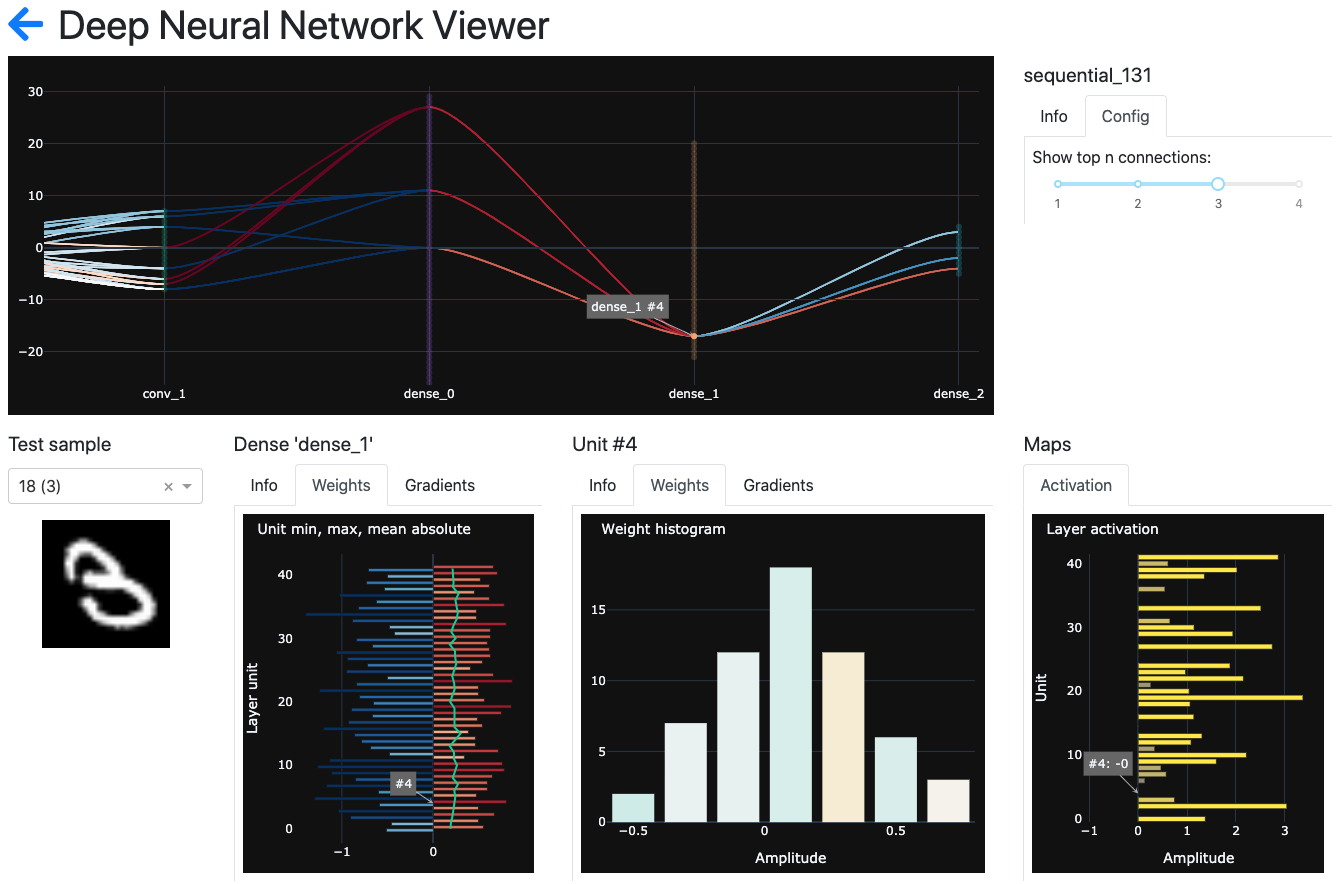
\includegraphics[scale=0.3]{images/dnn-viewer/BackwardThree_7.png}
    \caption{Backward exploration with a LeNet5, pre-softmax layer, unit \#4}
    \label{fig:dnn-viewer-backward-7}
\end{figure}

With this inspection, we have shown the potential of the DNN Viewer to quickly check and track the output of the network in order to understand some failures or fragile results. However, it has been quite difficult to find positive contributions to the softmax property being probed. In fact, the main view is showing only the top 3 main weights in absolute value, in this case all negative, and the layer weights are presented in the bottom panel as an histogram. This is room for improvement, one idea would be to add another view in this quadrant that mixes weights and activations to provide weighted contributions.

\subsubsection{Inspection over epochs}

For this inspection, used DNN is a classifier for the MNIST Fashion based on the Keras tutorial on CNN [\cite{keras-tutorial-cnn}]. This model was trained over 25 epochs as it is missing regularization, it is over-fitting as shown on Figure \ref{fig:dnn-viewer-time-training}.

\begin{figure}[H]
    \centering
    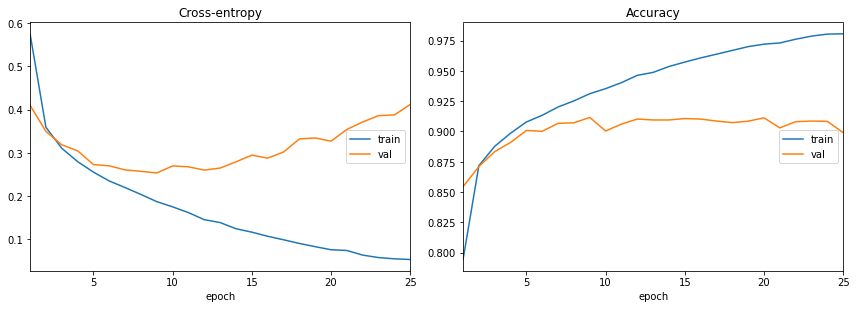
\includegraphics[scale=0.3]{images/dnn-viewer/Fashion-MNIST_Training.png}
    \caption{Training of the simple Fashion MNIST model}
    \label{fig:dnn-viewer-time-training}
\end{figure}

Using DNN Viewer, the activation of a test Shirt image is observed. Initially, softmax probability for the test sample is 70\% on the Shirt class. The gradient for the corresponding unit is relatively positive compared to other units of this layer.

\begin{figure}[H]
    \centering
    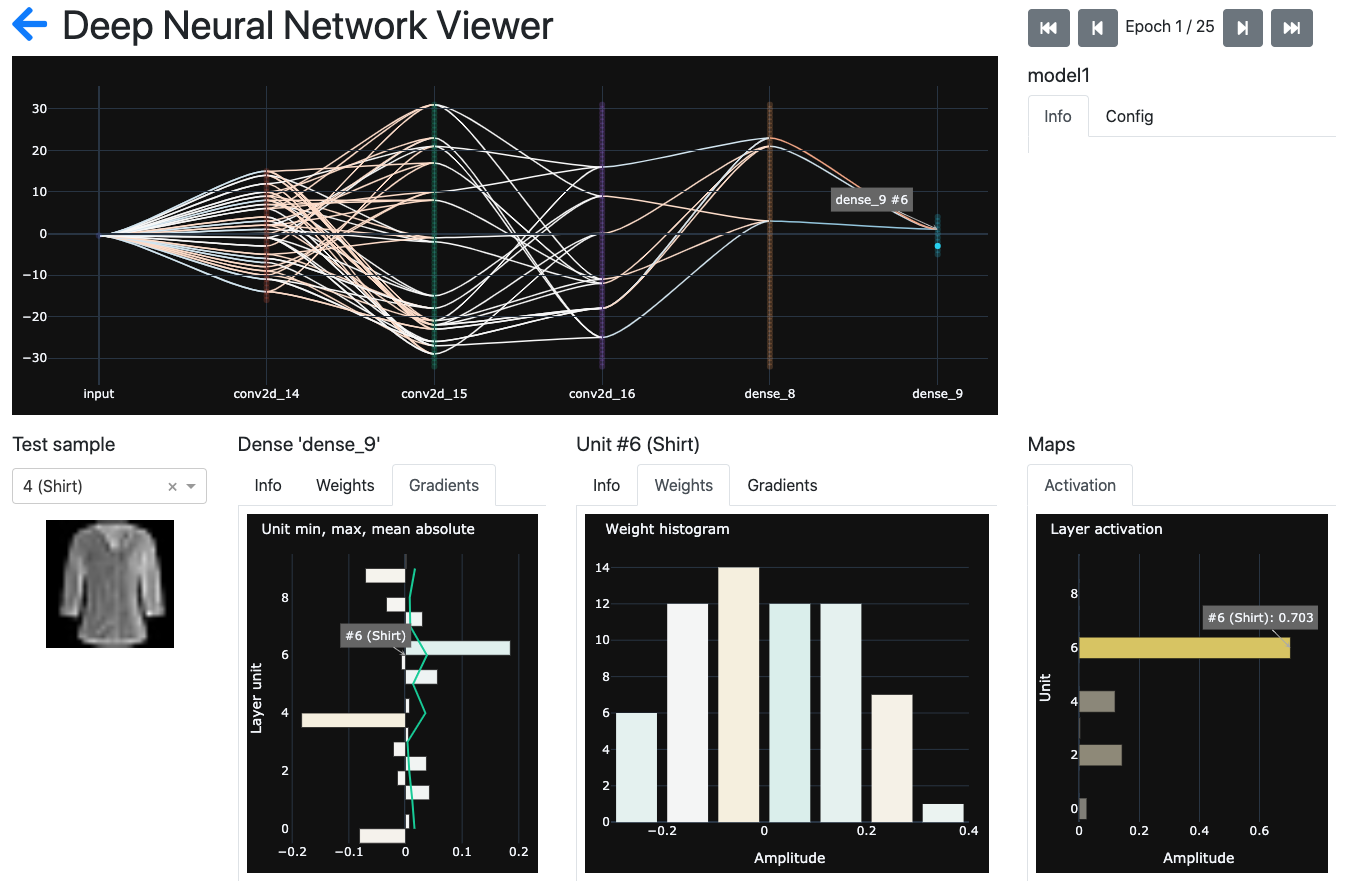
\includegraphics[scale=0.3]{images/dnn-viewer/TimeShirt_epoch1.png}
    \caption{Activation and weights for a Shirt test sample at epoch 1}
    \label{fig:dnn-viewer-time-shirt-epoch1}
\end{figure}

At the end of the epoch 2, the softmax probability has increased, gradient is still high.

\begin{figure}[H]
    \centering
    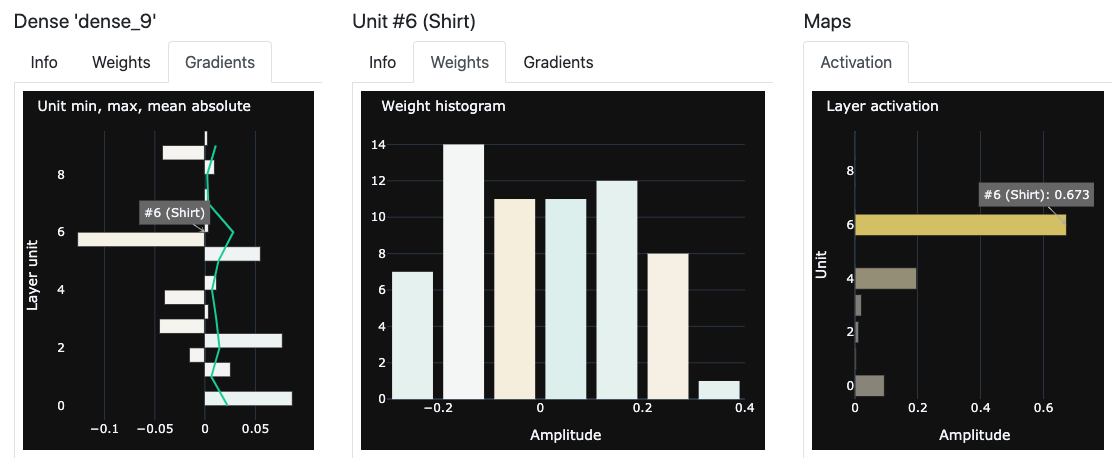
\includegraphics[scale=0.3]{images/dnn-viewer/TimeShirt_epoch3.png}
    \caption{Activation and weights for a Shirt test sample at epoch 2}
    \label{fig:dnn-viewer-time-shirt-epoch2}
\end{figure}

But at epoch 3, the softmax probability has decreased and the gradient is now mostly positive.

\begin{figure}[H]
    \centering
    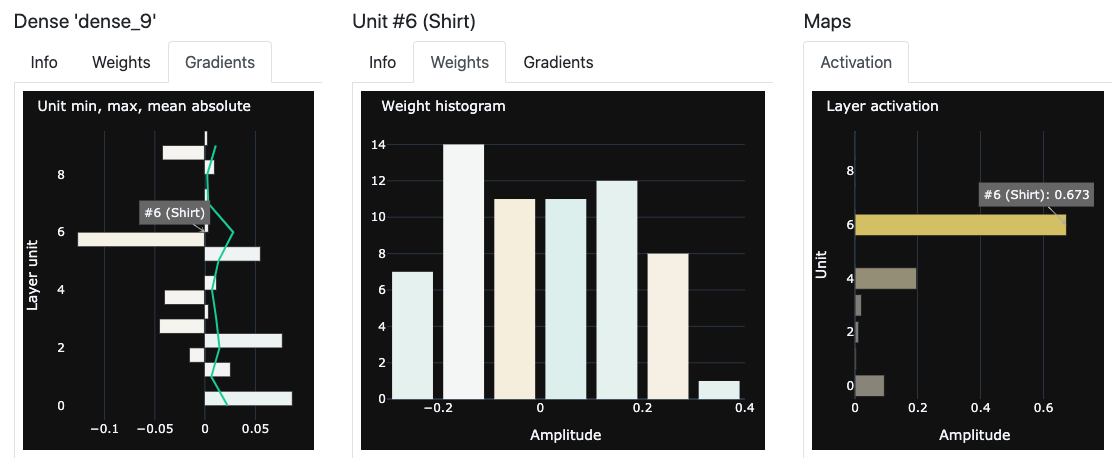
\includegraphics[scale=0.3]{images/dnn-viewer/TimeShirt_epoch3.png}
    \caption{Activation and weights for a Shirt test sample at epoch 3}
    \label{fig:dnn-viewer-time-shirt-epoch3}
\end{figure}

At epoch 4, the probability is raising again, gradients are more balanced.

\begin{figure}[H]
    \centering
    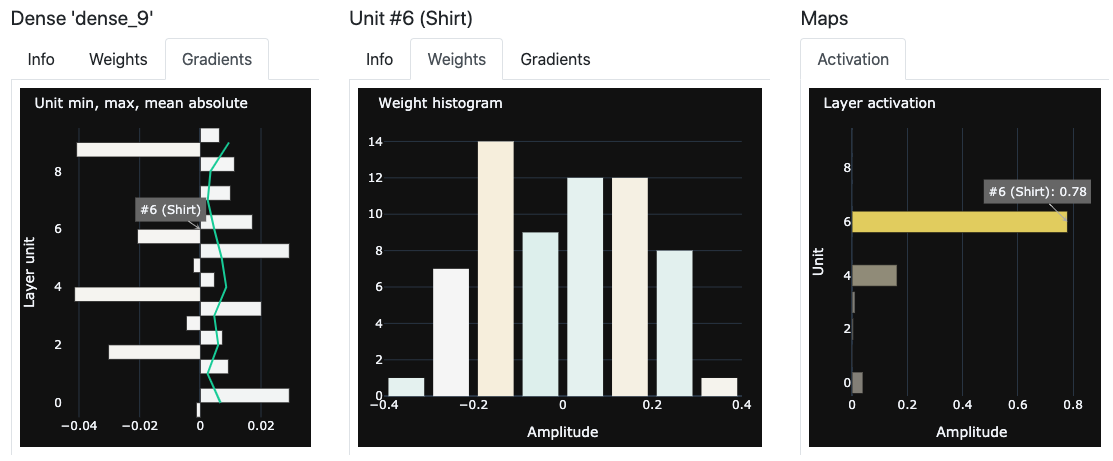
\includegraphics[scale=0.3]{images/dnn-viewer/TimeShirt_epoch4.png}
    \caption{Activation and weights for a Shirt test sample at epoch 4}
    \label{fig:dnn-viewer-time-shirt-epoch4}
\end{figure}

At epoch 5, the gradients are mostly positive and the probability is raising close to 90\%.

\begin{figure}[H]
    \centering
    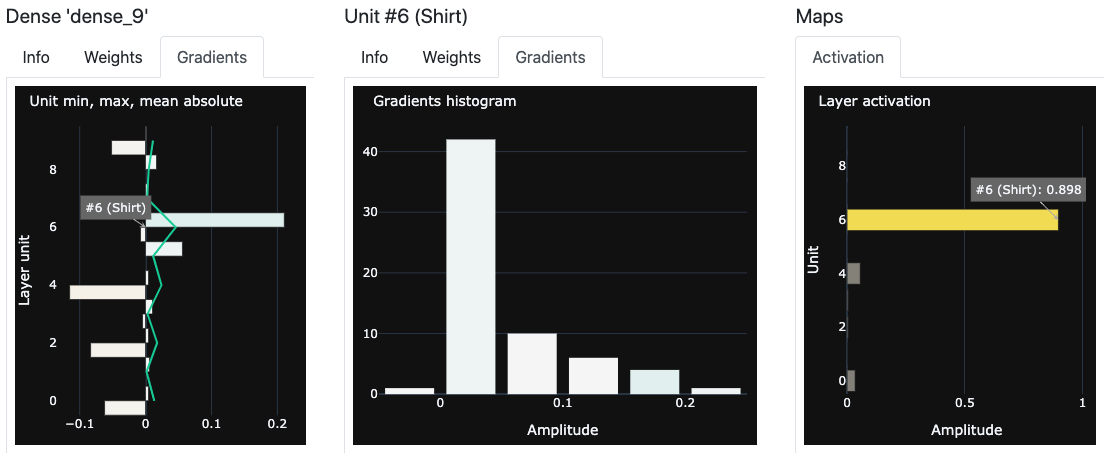
\includegraphics[scale=0.3]{images/dnn-viewer/TimeShirt_epoch5.png}
    \caption{Activation and weights for a Shirt test sample at epoch 5}
    \label{fig:dnn-viewer-time-shirt-epoch5}
\end{figure}

Jumping at epoch 8, the probability is a little lower, gradient are in majority at 0.

\begin{figure}[H]
    \centering
    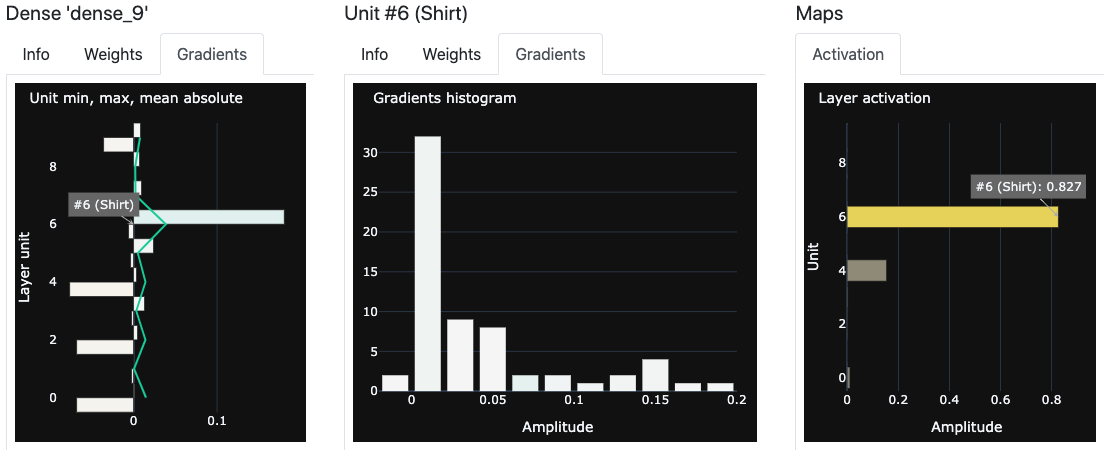
\includegraphics[scale=0.3]{images/dnn-viewer/TimeShirt_epoch8.png}
    \caption{Activation and weights for a Shirt test sample at epoch 8}
    \label{fig:dnn-viewer-time-shirt-epoch8}
\end{figure}

Jumping at epoch 15, the probability is very high at 96\%, gradient are in majority at 0, extrema are at +- 0.05.

\begin{figure}[H]
    \centering
    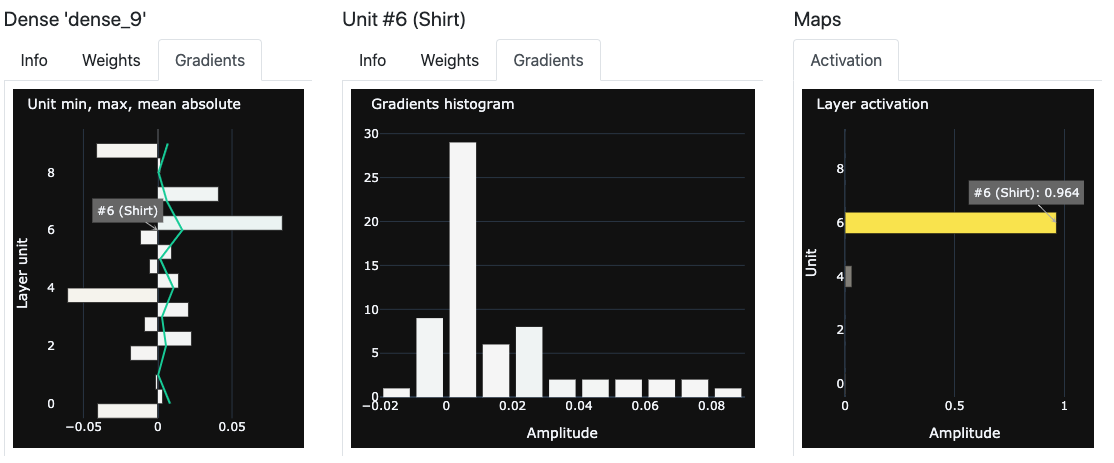
\includegraphics[scale=0.3]{images/dnn-viewer/TimeShirt_epoch15.png}
    \caption{Activation and weights for a Shirt test sample at epoch 15}
    \label{fig:dnn-viewer-time-shirt-epoch15}
\end{figure}

Eventually, at epoch 25, the performance is very good with a 99\% probability but the gradients extrema are still in the range of +- 0.1. We may think that the convergence is not completed, this is a consequence of the over-fitting.

\begin{figure}[H]
    \centering
    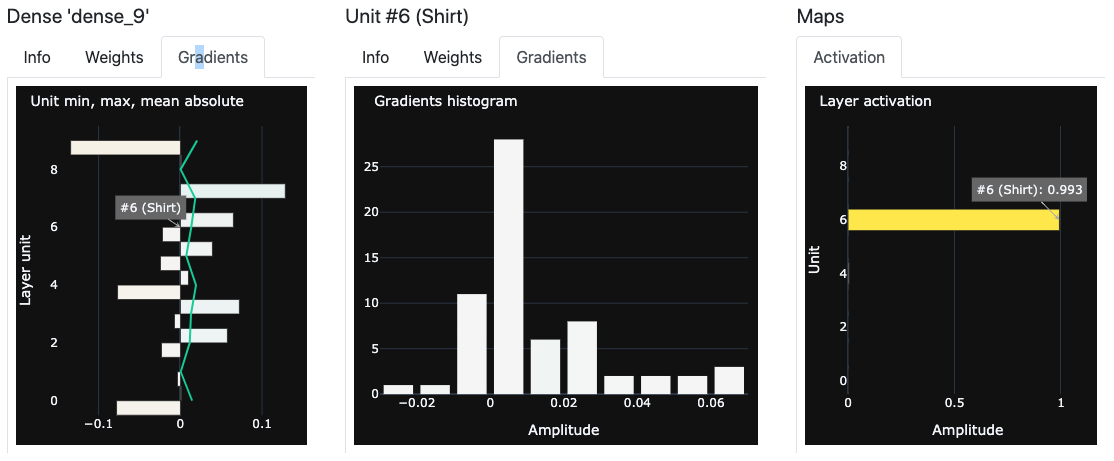
\includegraphics[scale=0.3]{images/dnn-viewer/TimeShirt_epoch25.png}
    \caption{Activation and weights for a Shirt test sample at epoch 25}
    \label{fig:dnn-viewer-time-shirt-epoch25}
\end{figure}



\subsection{DNN Viewer improvements and new features in P4}

During the last period, the DNN Viewer has been refined with many bug fixes and with improvements to support more models. Opening DNN Viewer as a generic tool to view saved models is quite a challenge given the huge amount of options on layers (strides, regularizations), the many types of layers (dense, convolutional 1D/2D/3D, pooling max/average 1D/2D/3D, activations, batch normalization...), the versions of Tensorflow (2.0, 2.1, 2.2) and format types (HDF5, checkpoints). The coming version of DNN Viewer is much stronger and versatile even if still not supporting all layer types.

During the period, the scope of the DNN Viewer has been enlarged with the following features and tests:
\begin{itemize}
    \item More descriptive properties to the network and to the layers
    \item Support for Tensorflow Data-sets
    \item Support for more layers, enabling GAN networks (including the Sequential within Sequential topology)
\end{itemize}


\begin{figure}[H]
    \centering
    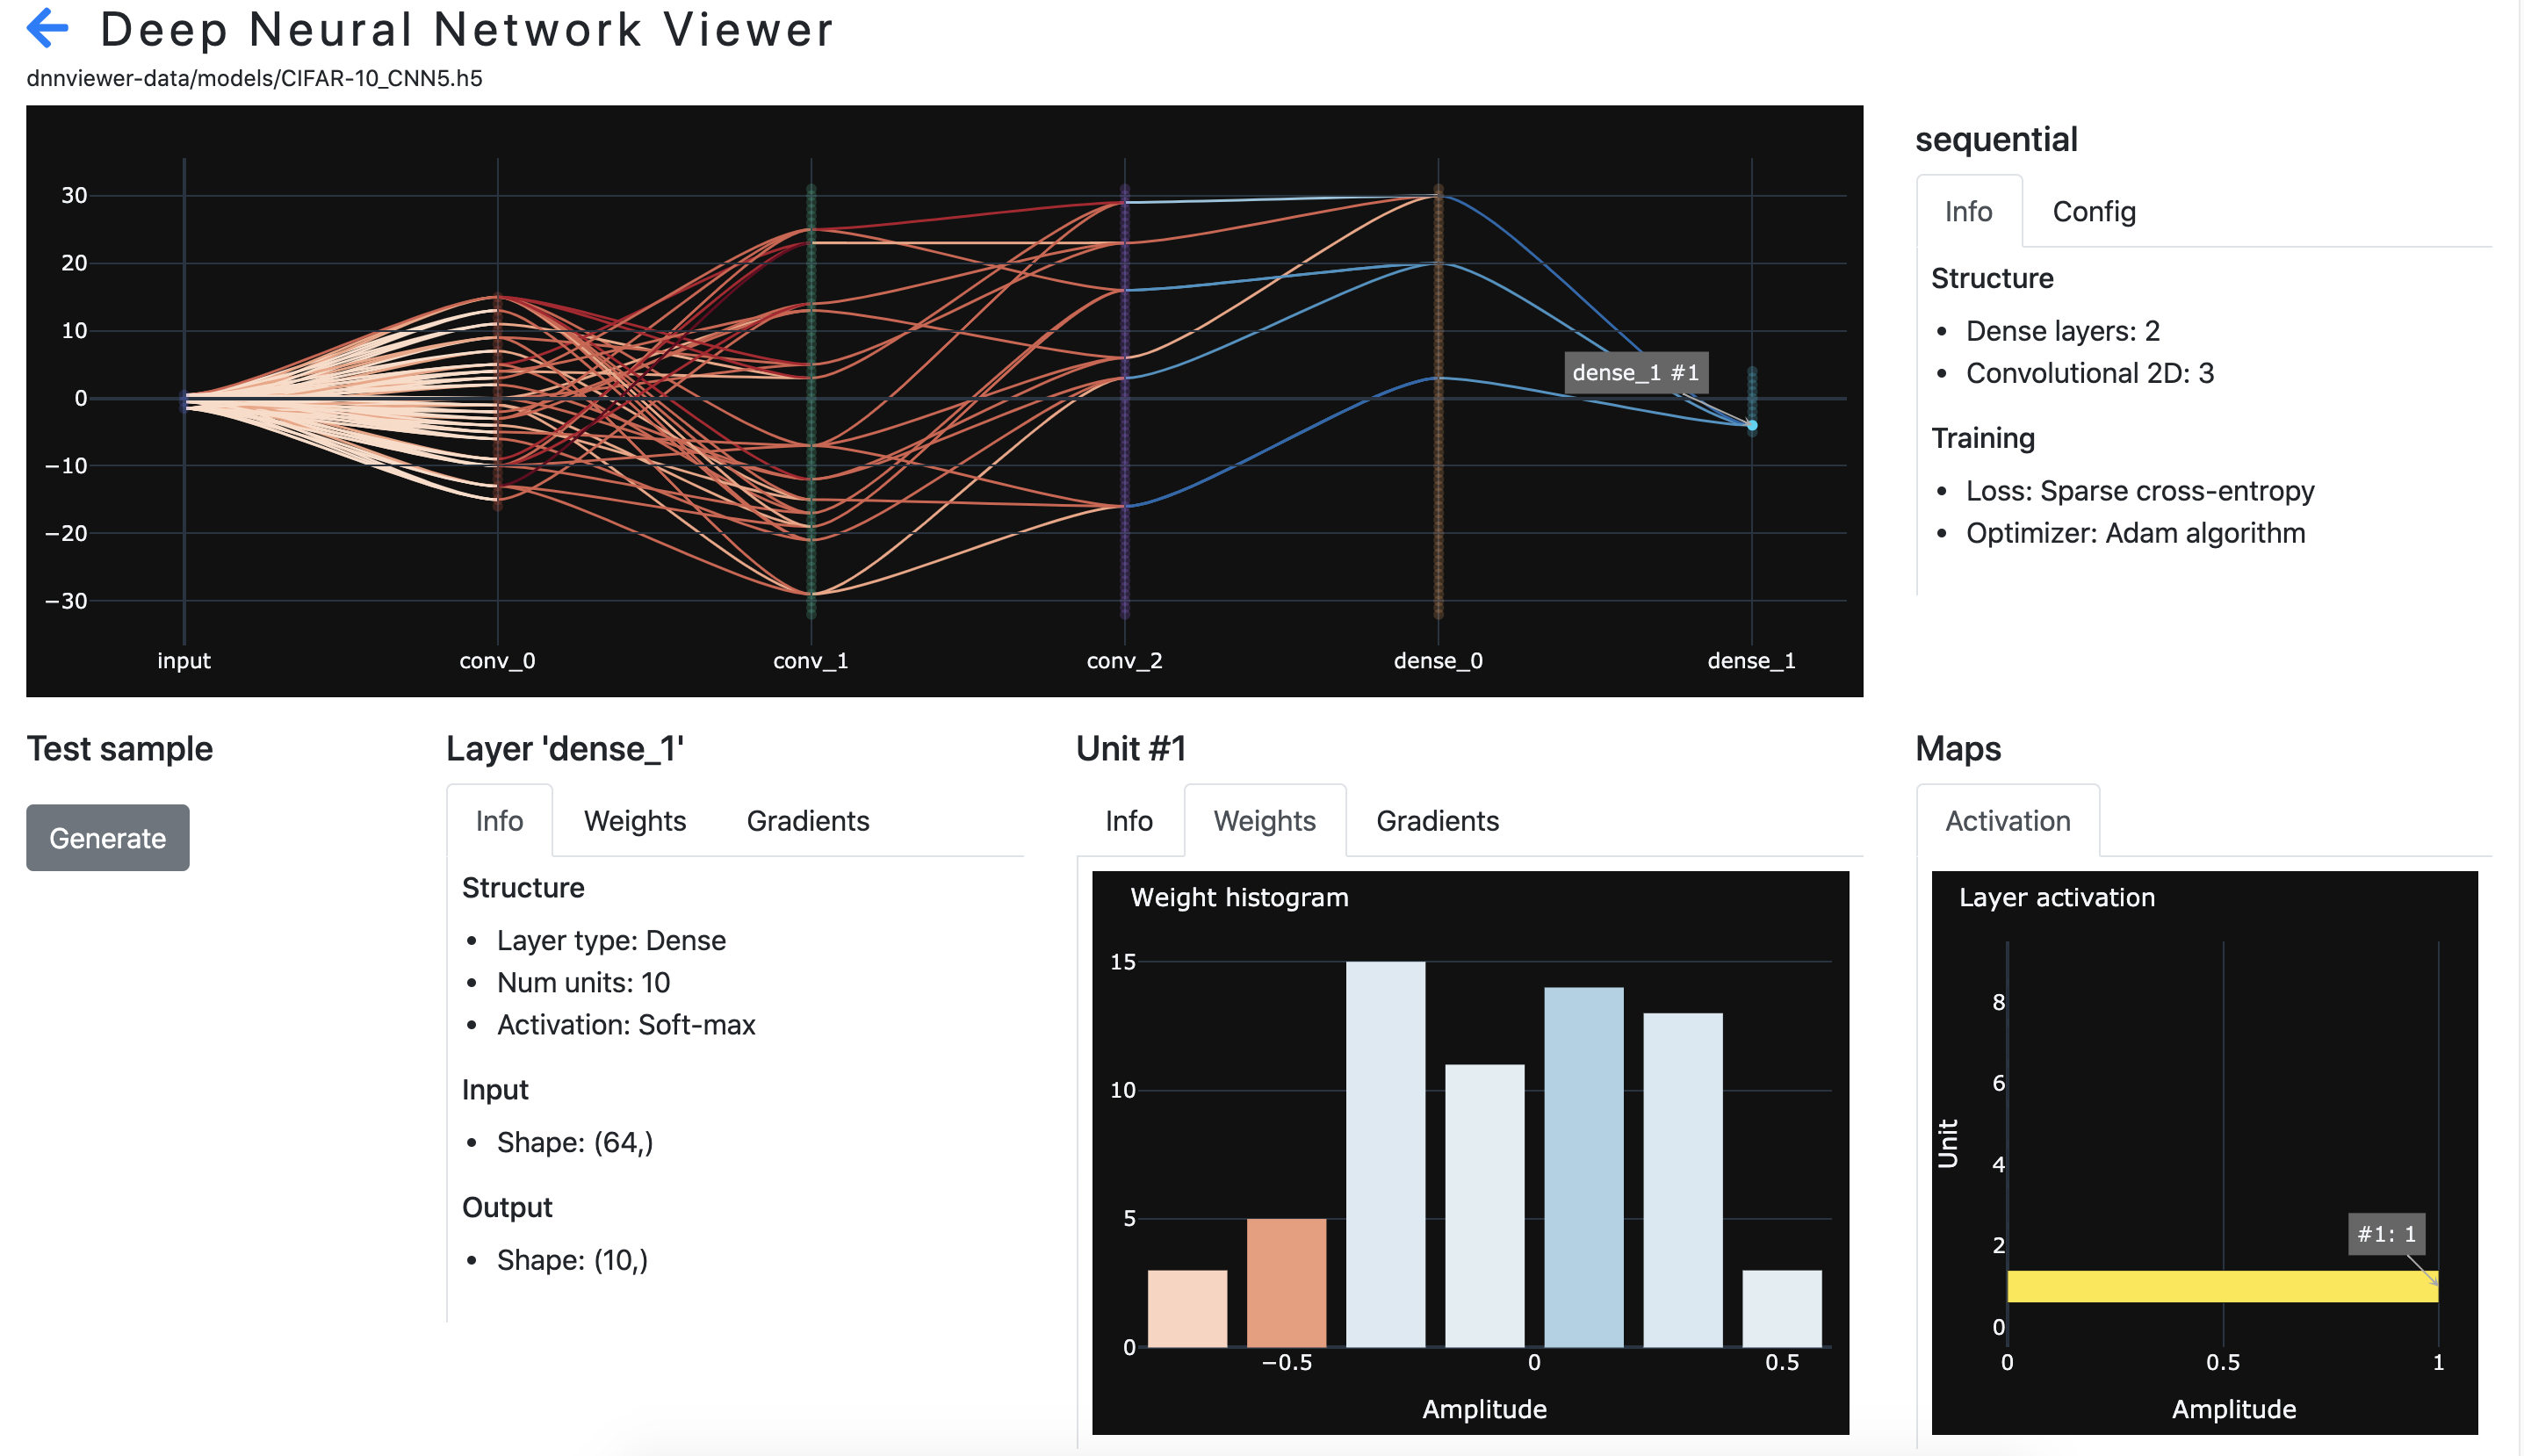
\includegraphics[scale=0.3]{images/dnn-viewer/CIFAR10+Random.png}
    \caption{Using the random generator as input on a CIFAR10 classifier is showing that class 1 (car) has probability 1, this result is reproducible. Does it mean that random noise is a car?}
    \label{fig:dnn-viewer-random-generator-cifar10}
\end{figure}

We have also been looking for feedback from users. A survey has been submitted to the students of the MS BigData, and to the machine learning teachers. Two students and two teachers have answered to the survey, among which two have succesfully tested the software, and with high interest. The main shared feedback is to provide more datasets, or capabilities to load personal datasets. Looking at the online feedback, even if Pipy is reporting more than 1000 downloads per mont since April, DNN Viewer is still looking for its public and more communication is required to advertise it.



\subsection{DNN Viewer next steps}

The DNN viewer is now an open source project on Github [\cite{dnnviewer2020}] and the package is distributed through Pip.org [\cite{dnnviewer-pypi2020}]. You may already install it and try it with your own "baby models".

As said in previous section, DNN Viewer needs to find a public of users, and ultimatly a community. Along with the improvements listed below, we will actively promote it on the Internet. The first step being a publication on Medium to present the software, its capabilities.

Incremental improvements:
\begin{itemize}
    \item Saliency as an alternative to activation maps
    \item More configuration to the views and better view when the view is complex (e.g. convolutional unit filter number may be large)
    \item Training loss and metrics Graphs
    \item Support for personal data-sets
    \item Improve on the visualization of the contributions as suggested above
\end{itemize}

Extensions to the tool:
\begin{itemize}
    \item Support for more complex architectures like residual networks
    \item Support for other tasks: NLP, time series, recurrent networks...
    \item More complex views and statistics that would require asynchronous server processing: UMAP (see \ref{sec5}), Intersection over Union [\cite{Zhou2017}]
\end{itemize}

Last but probably not least, at this point in the software development of DNN Viewer, we think that Dash is probably not the best tool to design a complete single page application, we are thinking of rebuilding it in a two tier architecture with Flask on the server, and a client side (browser) app built directly on React.js and Plotly.js.